% #########################################################################
% ##                          FITXER: 8_resultats.tex                    ##
% ##                     Contingut: Capítol de resultats                 ##
% #########################################################################

\documentclass[../main.tex]{subfiles}

% ------------------------------------------------------------
% Paquets específics
% ------------------------------------------------------------
\usepackage{paquets_format}
%\usepackage{almutils}

% ------------------------------------------------------------
% Inici del document
% ------------------------------------------------------------
\begin{document}

% ============================================================
% CAPÍTOL: Results
% ============================================================

\chapter{Avaluació comparativa dels models} \label{ch:results_comparativa_models}

Un cop seleccionats els millors models de cada enfocament, es comparen directament els resultats obtinguts amb SARIMA \texttt{C1} i LSTM \texttt{Exp6}. A la \cref{tab:comp_millor_arima_lstm} es mostren les mètriques d’error per a cada model, mentre que la \cref{fig:comp_arima_lstm}  permet visualitzar les prediccions i l’error absolut acumulat al llarg del període.

Els resultats mostren que ARIMA dona millors mètriques en tots els casos, amb una diferència notable en RMSE i MSE. El gràfic també ho confirma: tots dos models segueixen força bé la tendència, però el SARIMA ajusta millor les oscil·lacions i genera menys error acumulat. L’LSTM, en canvi, tendeix a desviar-se lleugerament a mesura que reutilitza les seves pròpies prediccions.

Aquest comportament s’explica per la naturalesa de la sèrie, que és força estable, amb una estacionalitat diürna molt marcada i un component aleatori relativament suau. En aquest context, un model clàssic com el SARIMA ja és capaç de capturar les principals tendències amb una bona precisió. Ara bé, en escenaris més complexos, com poden ser estacions de fons de vall, amb major presència de fenòmens no lineals, inversions tèrmiques abruptes o canvis sobtats de règim meteorològic, és probable que els models LSTM puguin oferir avantatges més clars. 

\begin{table}[H]
    \centering
    \small
    \renewcommand{\arraystretch}{1.2}
    \begin{tabular}{lcccc}
        \toprule
        \textbf{Model} & \textbf{ID} & \textbf{RMSE} & \textbf{MSE}& \textbf{MAE}\\
        \midrule
        ARIMA & C1& 1.3144& 1.7279& 0.9371\\
        LSTM  & Exp 6& 1.52& 2.3104& 1.0436\\
        \bottomrule
    \end{tabular}
    \caption{Comparativa de les mètriques d’error entre els millors models ARIMA i LSTM seleccionats.}
    \label{tab:comp_millor_arima_lstm}
\end{table}

\begin{figure}[H]
    \centering
    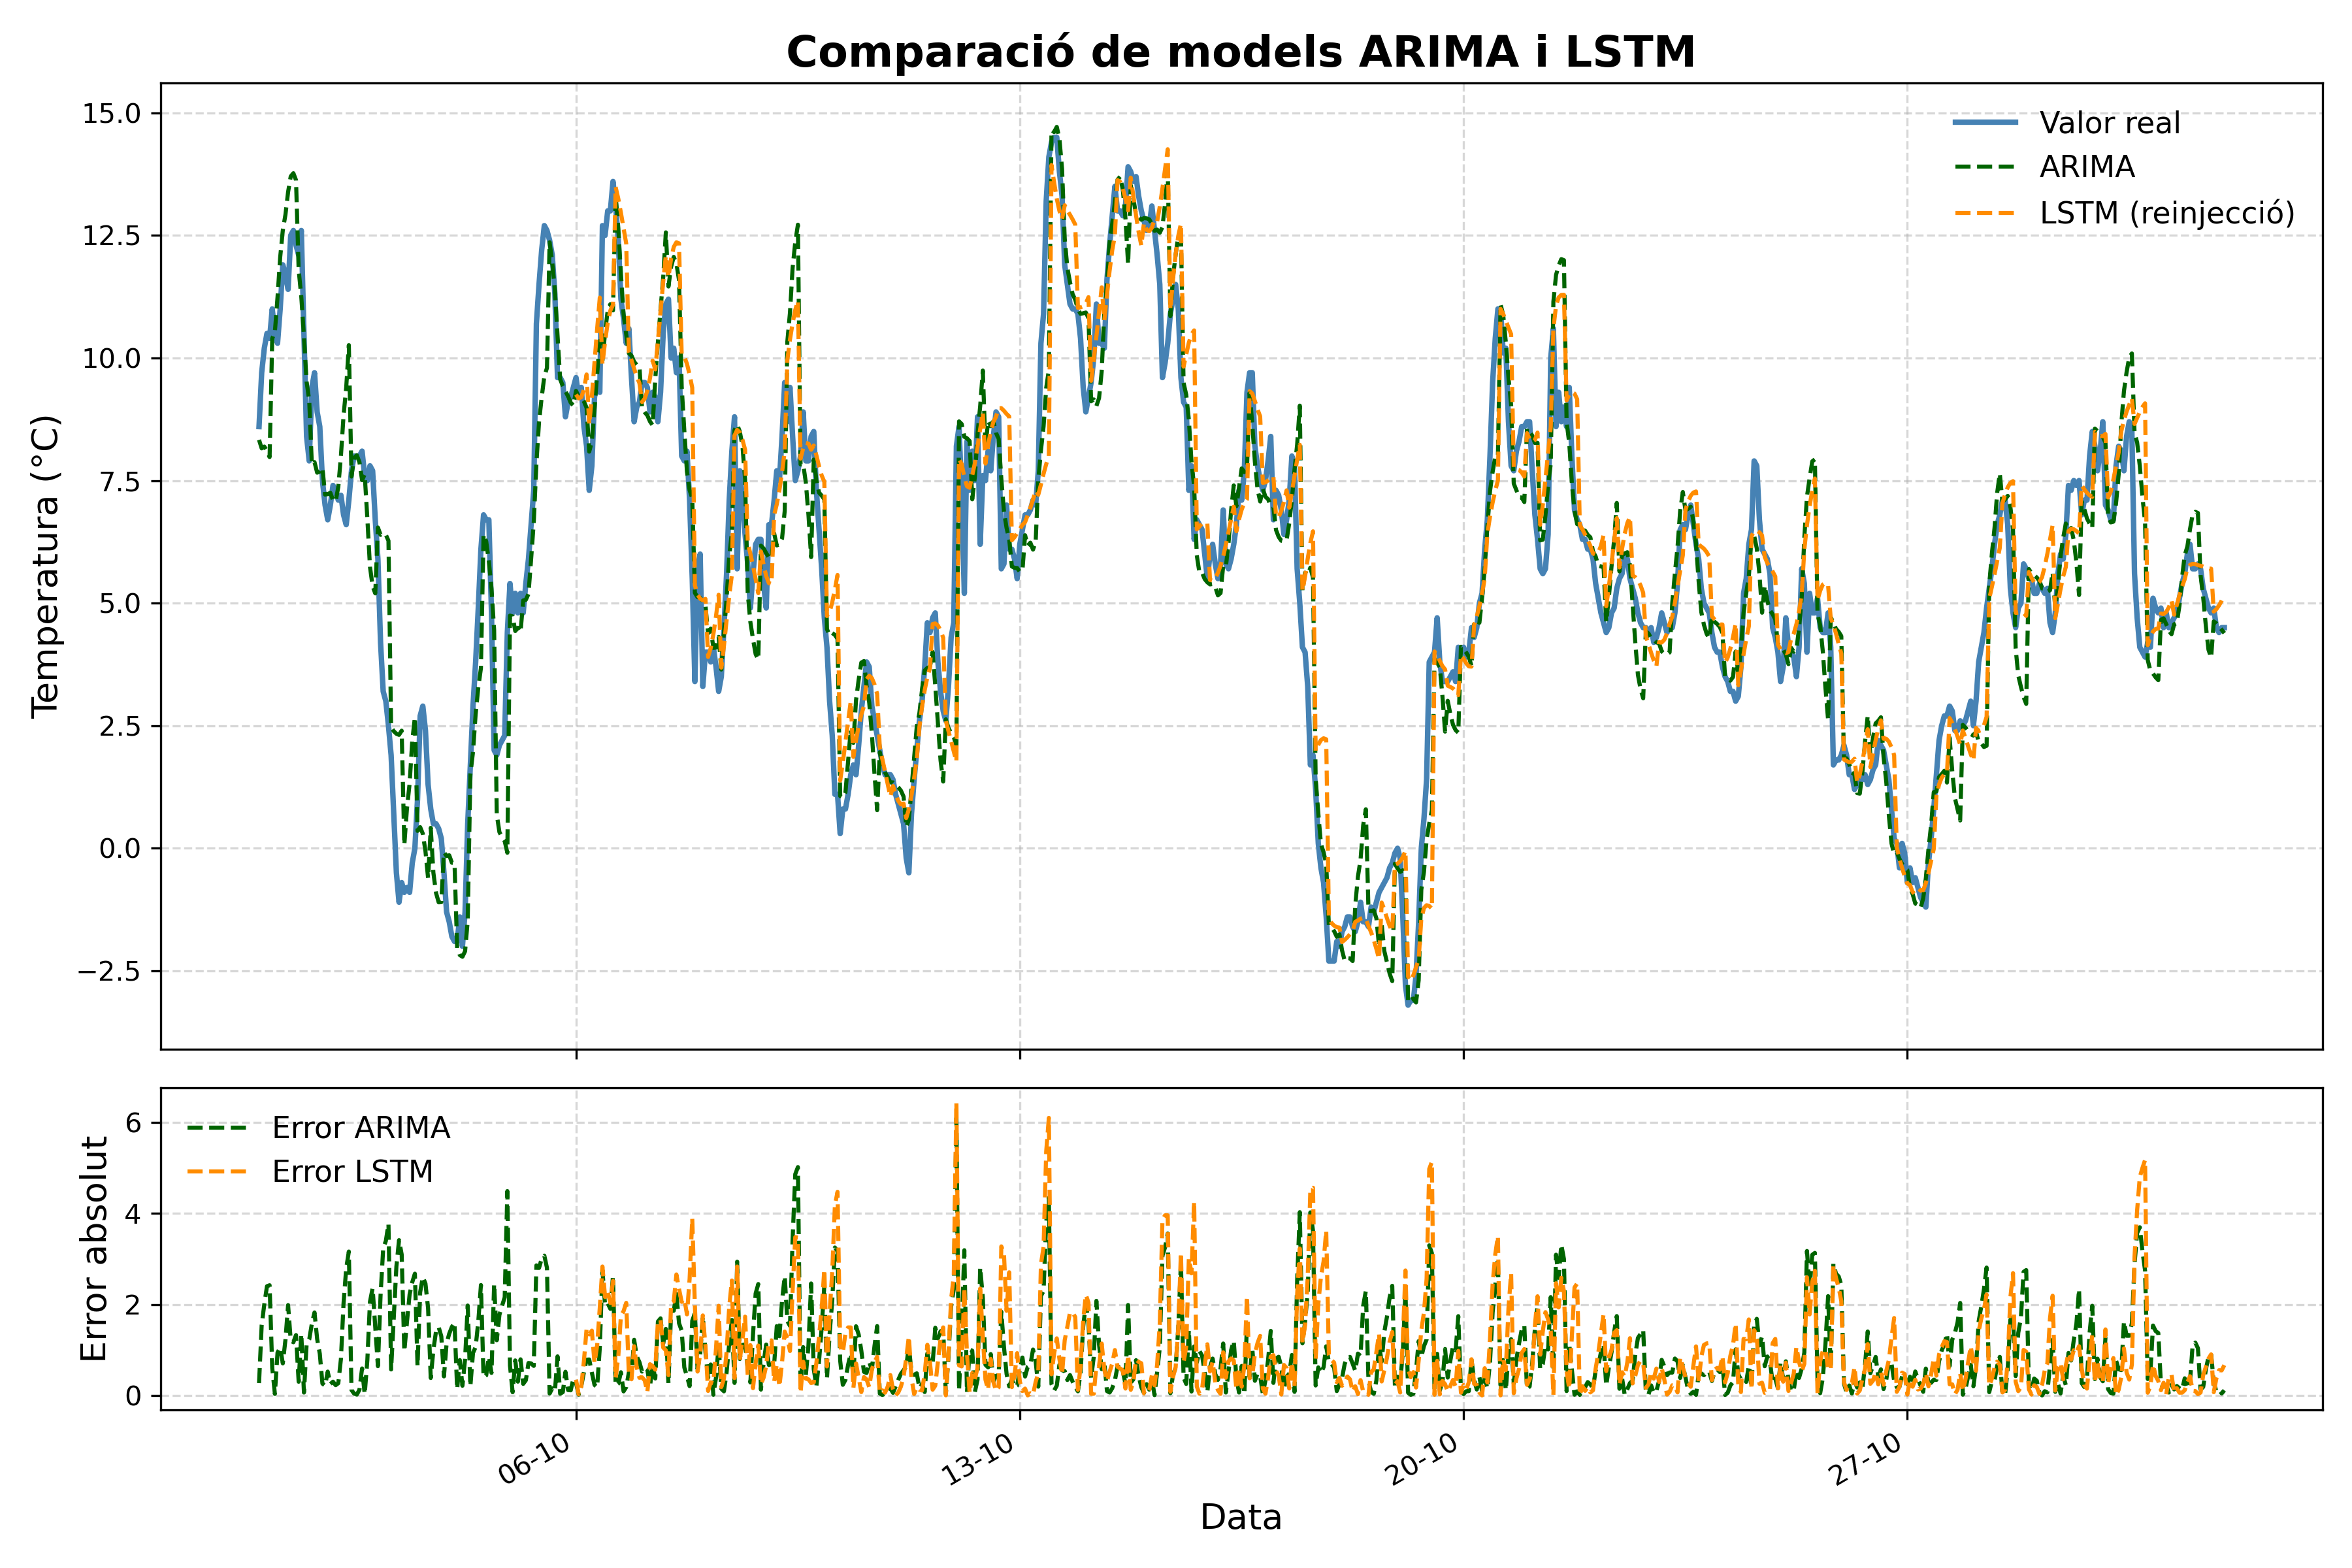
\includegraphics[width=0.75\linewidth]{figures/comp_arima_lstm/comparacio_models_amb_errors.png}
    \caption{Comparació de les prediccions i errors absoluts entre models ARIMA i LSTM }
    \label{fig:comp_arima_lstm}
\end{figure}


% ------------------------------------------------------------
% Fi del document
% ------------------------------------------------------------
\end{document}
